\let\negmedspace\undefined
\let\negthickspace\undefined
\documentclass[journal]{IEEEtran}
\usepackage[a5paper, margin=10mm, onecolumn]{geometry}
%\usepackage{lmodern} % Ensure lmodern is loaded for pdflatex
\usepackage{tfrupee} % Include tfrupee package

\setlength{\headheight}{1cm} % Set the height of the header box
\setlength{\headsep}{0mm}     % Set the distance between the header box and the top of the text

\usepackage{gvv-book}
\usepackage{gvv}
\usepackage{cite}
\usepackage{amsmath,amssymb,amsfonts,amsthm}
\usepackage{algorithmic}
\usepackage{graphicx}
\usepackage{textcomp}
\usepackage{xcolor}
\usepackage{txfonts}
\usepackage{listings}
\usepackage{enumitem}
\usepackage{mathtools}
\usepackage{gensymb}
\usepackage{comment}
\usepackage[breaklinks=true]{hyperref}
\usepackage{tkz-euclide} 
\usepackage{listings}
% \usepackage{gvv}                                        
\def\inputGnumericTable{}                                 
\usepackage[latin1]{inputenc}                                
\usepackage{color}                                            
\usepackage{array}                                            
\usepackage{longtable}                                       
\usepackage{calc}                                             
\usepackage{multirow}                                         
\usepackage{hhline}                                           
\usepackage{ifthen}                                           
\usepackage{lscape}
\begin{document}

\bibliographystyle{IEEEtran}
\vspace{3cm}

\title{1.1.4.5}
\author{EE24BTECH11030 - J.KEDARANANDA
}
% \maketitle
% \newpage
% \bigskip
{\let\newpage\relax\maketitle}

\renewcommand{\thefigure}{\theenumi}
\renewcommand{\thetable}{\theenumi}
\setlength{\intextsep}{10pt} % Space between text and floats


\numberwithin{equation}{enumi}
\numberwithin{figure}{enumi}
\renewcommand{\thetable}{\theenumi}


\textbf{Question}:\\
Find the coordinates of $\vec{P}$ on $\vec{AD}$ such that $\vec{AP:PD}=2:1.$where coordinates of $\vec{A}$ are $\brak{0,0}$ and $\vec{B}$ are $\brak{0,9}$
\\
\textbf{Solution: }
\begin{table}[h!]    
  \centering
  \begin{center}
    \begin{tabular}{|c|c|} 
        \hline
            \textbf{Variable} & \textbf{Value} \\ 
        \hline
            $\boldsymbol{BC}$ & 6 cm \\ 
        \hline
            $\boldsymbol{AB}$ & 5 cm \\ 
        \hline
            $\angle \vec{B}$  & $60^\circ$ \\
        \hline
    \end{tabular}
\end{center}  



  \caption{Variables Used}
  \label{tab10.5.3.9.1}
\end{table}
According to the question as $\vec{P}$ divides $\vec{AB}$ in the ratio 2:1 we can write\\
\begin{align}
\vec{P}=\frac{k(\vec{B})+(\vec{A})}{k+1}=\myvec{x\\y}\\
\end{align}
where the value of k mentions about the ratio in which $\vec{P}$ divides $\vec{AB}$\\
Here according to problem value of k is 2\\
\begin{align}
P=\frac{2B+A}{3}=\frac{3\myvec{0\\9}+\myvec{0\\0}}{3}=\frac{\myvec{0\\18}}{3}\\
\end{align}
\begin{align}
P=\myvec{0\\6}
\end{align}
with simple comparison we can say that 
\begin{align}
x=0\\
y=6\\
\end{align}
Hence the coordinates of $\vec{P}$ are $\brak{0,6}$
\begin{figure}[h!]
   \centering
   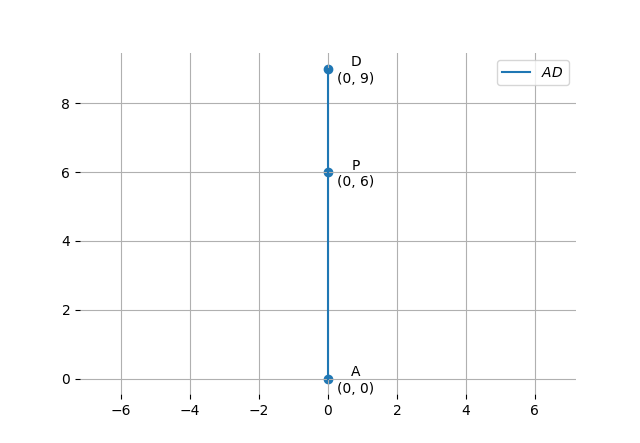
\includegraphics[width=0.7\linewidth]{figs/Fig1.png}
   \caption{Stem Plot of y\brak{n}}
   \label{stemplot}
\end{figure}
\end{document}  
\end{document}
